\documentclass[a4paper,12pt,oneside,final]{article}
\usepackage[pdftex]{graphicx}
\usepackage[T1]{fontenc}
\usepackage{titlesec, color}
\usepackage{anysize}
\usepackage{listings}

\newenvironment{changemargin}[2]{\begin{list}{}{%
\setlength{\topsep}{0pt}%
\setlength{\leftmargin}{0pt}%
\setlength{\rightmargin}{0pt}%
\setlength{\listparindent}{\parindent}%
\setlength{\itemindent}{\parindent}%
\setlength{\parsep}{0pt plus 1pt}%
\addtolength{\leftmargin}{#1}%
\addtolength{\rightmargin}{#2}%
}\item }{\end{list}}
\marginsize{30mm}{30mm}{20mm}{20mm}
\definecolor{gray75}{gray}{0.75}
\newcommand{\hsp}{\hspace{20pt}}
\author{
    Yufei Wang (yw6312, s5) \\ 
    Paul Gribelyuk (pg1312, a5) \\
    Yawei Li (yl8012, s5) \\ 
    Jun He (jh1212, s5) \\
    Xiaoxing Yang (xy212, s5)
}
\makeatother

\title{\Huge Software Engineering for Industry \\ Coursework 2: AcmeTelecom Billing System}

\begin{document}
\maketitle

\section{Introduction} % paul
This report covers the analysis, testing, refactoring, and re-engineering of the AcmeTelecom billing system.  We saw our responsibility as two-fold: to build a well-tested, easy to maintain, coherent piece of software, and to use that software to implement a billing algorithm which fairly bills clients according to the time they spent calling during peak and off-peak times.  We relied heavily on Test Driven Development (TDD) practices in the way we devised tests, using unit tests to assert the state of our system, and mock tests to verify its behaviour.  To put in place tests for the initial code base, we were forced to make decisions about design patterns present (such as the singleton pattern in \verb+HtmlPrinter+) as well as make heavy use of interfaces to allow the JMock libraries to interact with out code.  Once satisfied with the initial functionality, we wrote integration tests and opened the development process to the business expert by writing a DSL around the components most responsible for how the billing system determines rates for customers.

We used these specificaitons to guide us in the design phase, where we ultimately chose to preserve the structure of the \verb+BillingSystem+ object as the class which is the central component collecting call information and passing them on to the \verb+BillGenerator+ rather than deciding what those calls shoudl cost.  We externalized that business logic by putting it in a separate class, thus making the original class more cohesive and simplifying the process to incorporate future changes.  We used a modern version control system (\emph{git}) and a continous integration server to manage the testing framework and automatically build after each commit.  Dependency matrix analysis helped to gain a big-picture understanding of the codebase without reading every line.

We were also careful not to over-optimize and decided to keep the general design of the system in tact, since it also inter-operates with other external libraries throughout the AcmeTelecom organization.  If we were to implement a brand new design, we would have loosened the coupling further by using Dependency Inversion model wherever possible and definining how interfaces should communicate rather than how concrete classes should change state.
	

\section{Analysis of Original Code} % paul
The original code for the Billing System was well structured, though lacking any tests, so a look at the dependency structure was needed to begin to analyze where work would need to be done.  We have included a diagram of this here:
\begin{figure}[!h]
\begin{changemargin}{-20mm}{-20mm}
\center
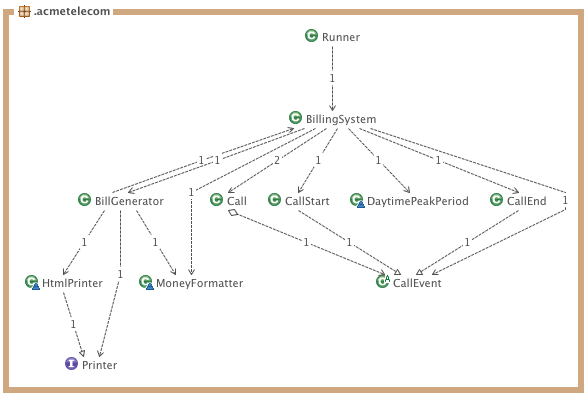
\includegraphics[scale=0.55]{Original_Structure.png}
\caption{Original Dependency Structure of the Billing System}
\end{changemargin}
\end{figure}i

The 3-layer architecture is preferable in this case, since it is an in-house system with a small well-defined userbase and more a intricate architecture pattern would not be needed. The code also lacks interfaces to begin to easily write tests, especially with JMock, which requires an interface to mock behaviour.  

The \verb+CallEvent+ is the basic building block of a \verb+Call+, which consists of a \verb+CallStart+ and a \verb+CallEnd+, which both inherit from \verb+CallEvent+.  The \verb+BillingSystem+ receives method calls to \verb+callInitiated+ and \verb+callCompleted+ and logs them to a \verb+List<>+ object.  A call to the \verb+createCustomerBills+ calculates the costs of each call as it occurs in teh list, and then dispatches this list of \verb+Calls+ to the \verb+BillGenerator+ by invoking \verb+send+.  The \verb+BillGenerator+ uses an \verb+HtmlPrinter+ to output the results into HTML (in this example, to \verb+System.out+).  Other classes, such as \verb+MoneyFormatter+ and \verb+DaytimePeakPeriod+ act as helper classes.

\section{Refactoring and Testing} % fred (maybe and paul)
Creating interfaces for testing purposes
Creating Mock tests
Creating Unit tests for container classes
Breaking \verb+HtmlPrinter+ singleton interface and changing constructor to take a different \verb+PrintStream+ other than \verb+System.out+.

Extracted calculation part of original \verb+BillingSystem+ into a new class to allow flexibility in future design.

\section{Creating a DSL} % fred

\section{Implementing the New Billing System}  % juno
% here we talk about the way to design new system and how the calculations happen
% include some important lines of code as examples



% \emph{emphasize} \textbf{boldface}

\section{Acceptance Tests} % cici and juno
\begin{itemize}
\item GivenPeakPeriod: 
\item GivenTheFollowingCustomers: 
\item GivenTheseCallsAreMade:
\item GivenTheSystemIsInitialized:
\item TheBillShows:
\end{itemize}

% \begin{figure}[!h]
% \begin{changemargin}{-20mm}{-20mm}
% \center
% \includegraphics[scale=1]{file_name.jpg}
% \caption{Caption string}
% \end{changemargin}
% \end{figure}i

\section{Conclusions and Recommendations} % leah
Tools used (Git, Jenkins, IntelliJ Coverage Report, IntelliJ Dependency Matrix).  Problems enountered like refactoring for Tiny Types, Mocking with concreted classes rather than interfaces.
% \blindtext
\end{document}
